\DailyTitle{6363 Log (November 17, 2010)}

\DailySection{Goals}

\begin{enumerate}
\item Test out the two round-3 candidate ideas
\item Code timing performance
\item Add reference to the hcal note
\end{enumerate}

\DailySection{Timing performance}

Did a test run on \texttt{Jet} dataset, run 149011, file \texttt{66A2FF37-3EE1-DF11-9934-0030487C8CBE.root} from \texttt{CASTOR} area.
10000 events run.  The result is shown in figure \ref{Figure_6363_JetDataset10000EventExecutionTime}.
Average execution time (CPU) for one event is roughly 1 ms.  Module \texttt{hbheprereco} is the standard Hcal reconstruction with fitting flags turned on.
Module \texttt{hbheprereconofitting} is the same thing except with fitting flags turned off.
Module \texttt{hbhereco} is the isolation-based flagging from JP.

\begin{figure}
   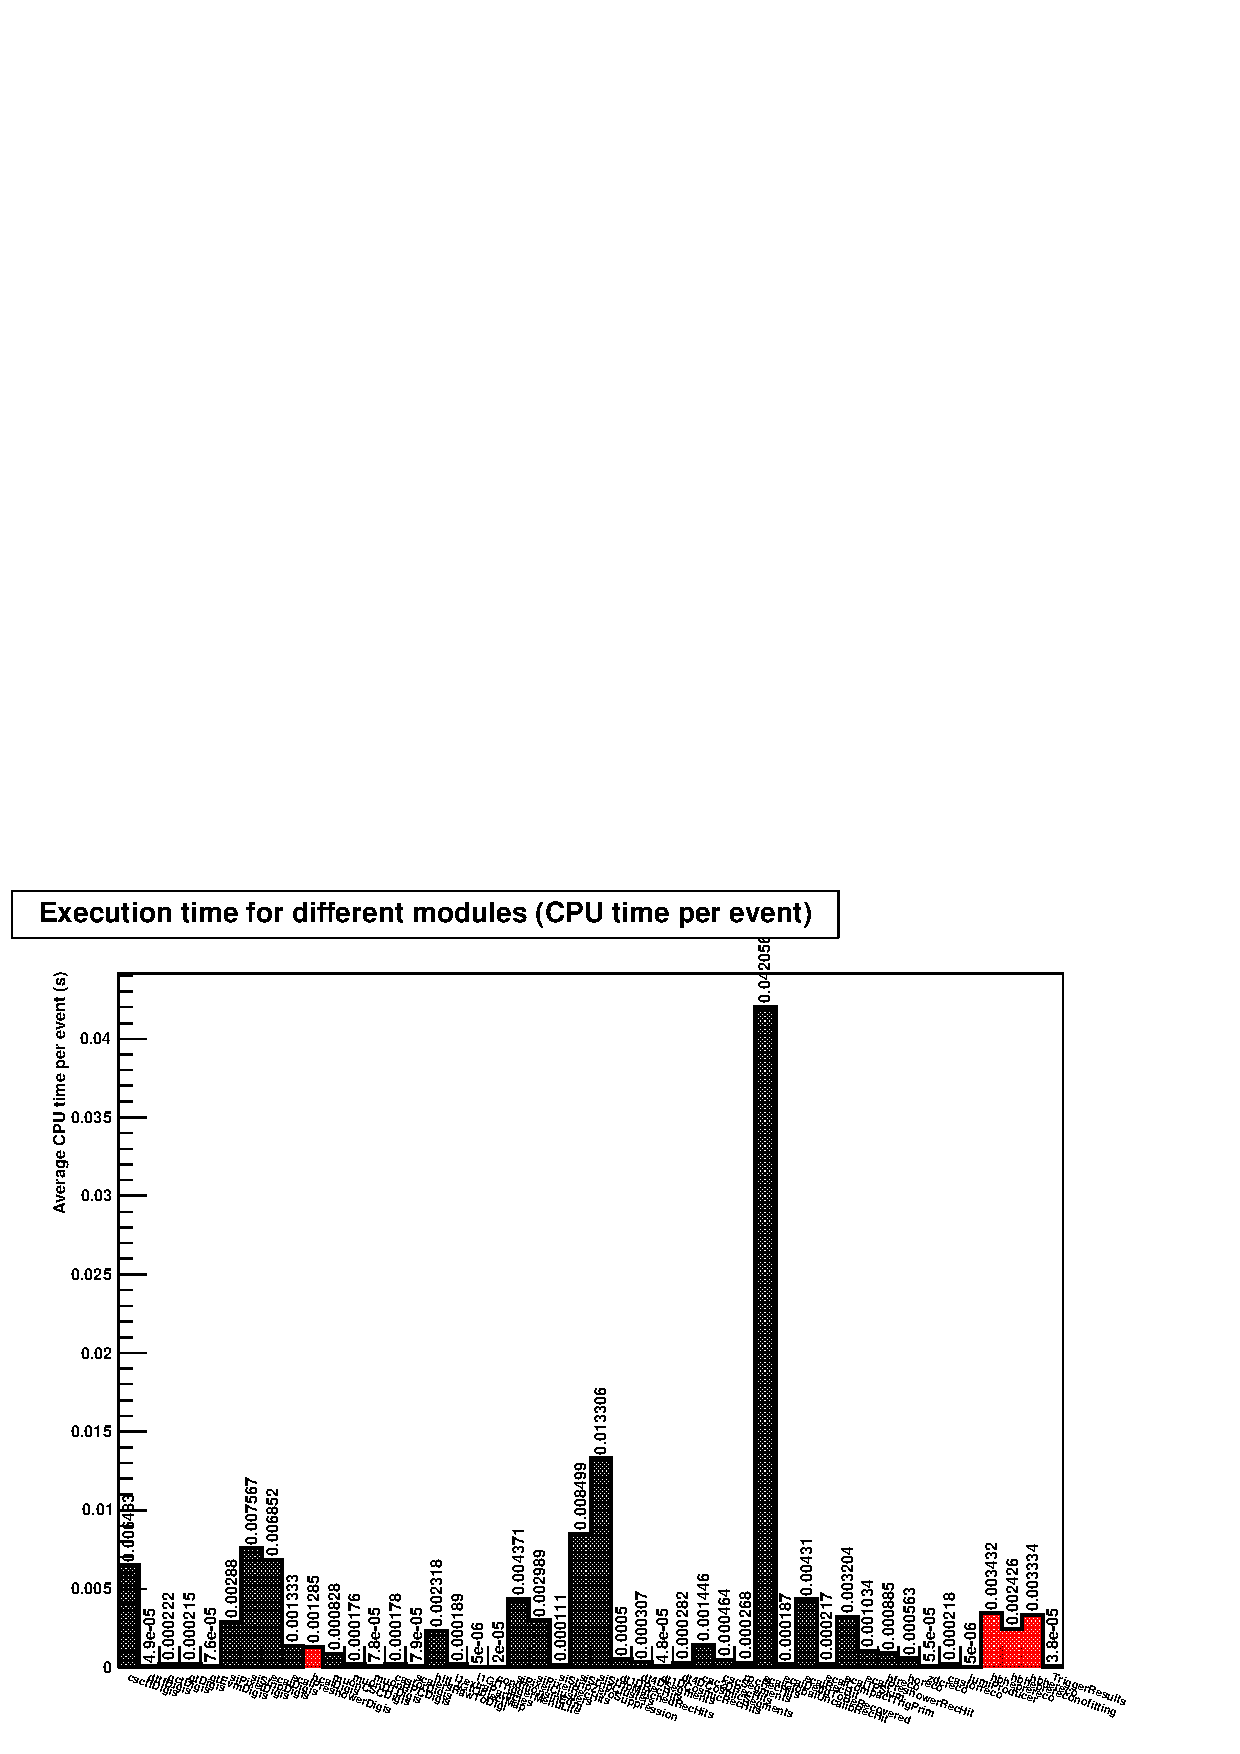
\includegraphics[width=120mm]{DailyLog/6363/6363_ExecutionTime.pdf}
   \caption{Average CPU time per event for \texttt{Jet} dataset, run 149011.}
   \label{Figure_6363_JetDataset10000EventExecutionTime}
\end{figure}

\DailySection{Action items for Hcal noise}

Talked briefly with Artur.  Needed to do

\begin{enumerate}
\item Smooth cut position curves.
\item Get timing envelope from Phil and test it.
\item MC?
\item Cleaned number of events?
\end{enumerate}


\DailySection{Preliminary plots for cleaning efficiency}

Take good noise events from the \texttt{HcalHPDNoise} sample, and plot the rechit energy distribution after each step of cleaning.
The distributions are shown in figure \ref{Figure_6363_RecHitEnergyDistributionCleaning}.
Rate of rechits remaining after cut is shown in figure \ref{Figure_6363_RecHitEnergyDistributionCleaningRatio}.

\begin{figure}
   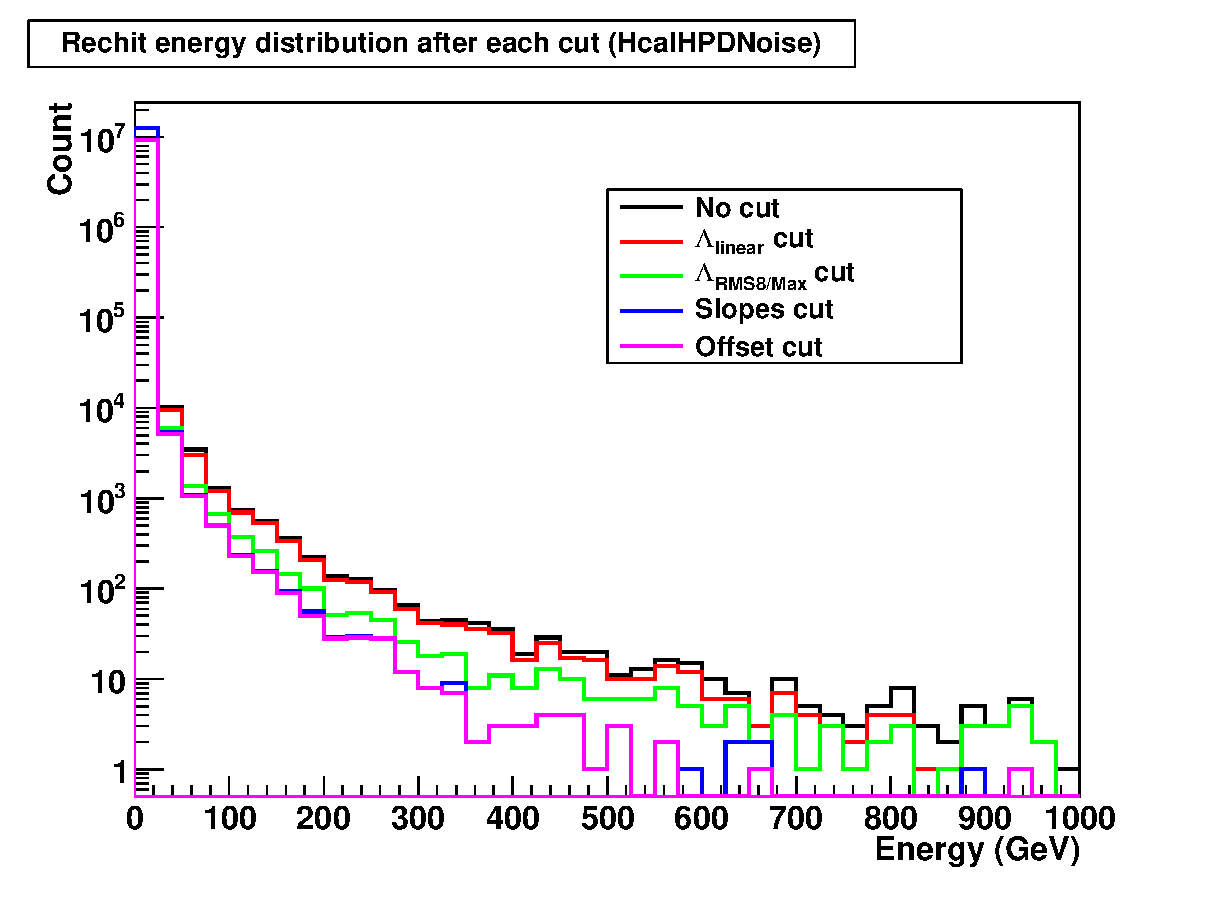
\includegraphics[width=120mm]{DailyLog/6363/6363_RecHitEnergyComparisonPlot_HcalHPDNoise}
   \caption{Rechit energy distribution after each step of cleaning}
   \label{Figure_6363_RecHitEnergyDistributionCleaning}
\end{figure}

\begin{figure}
   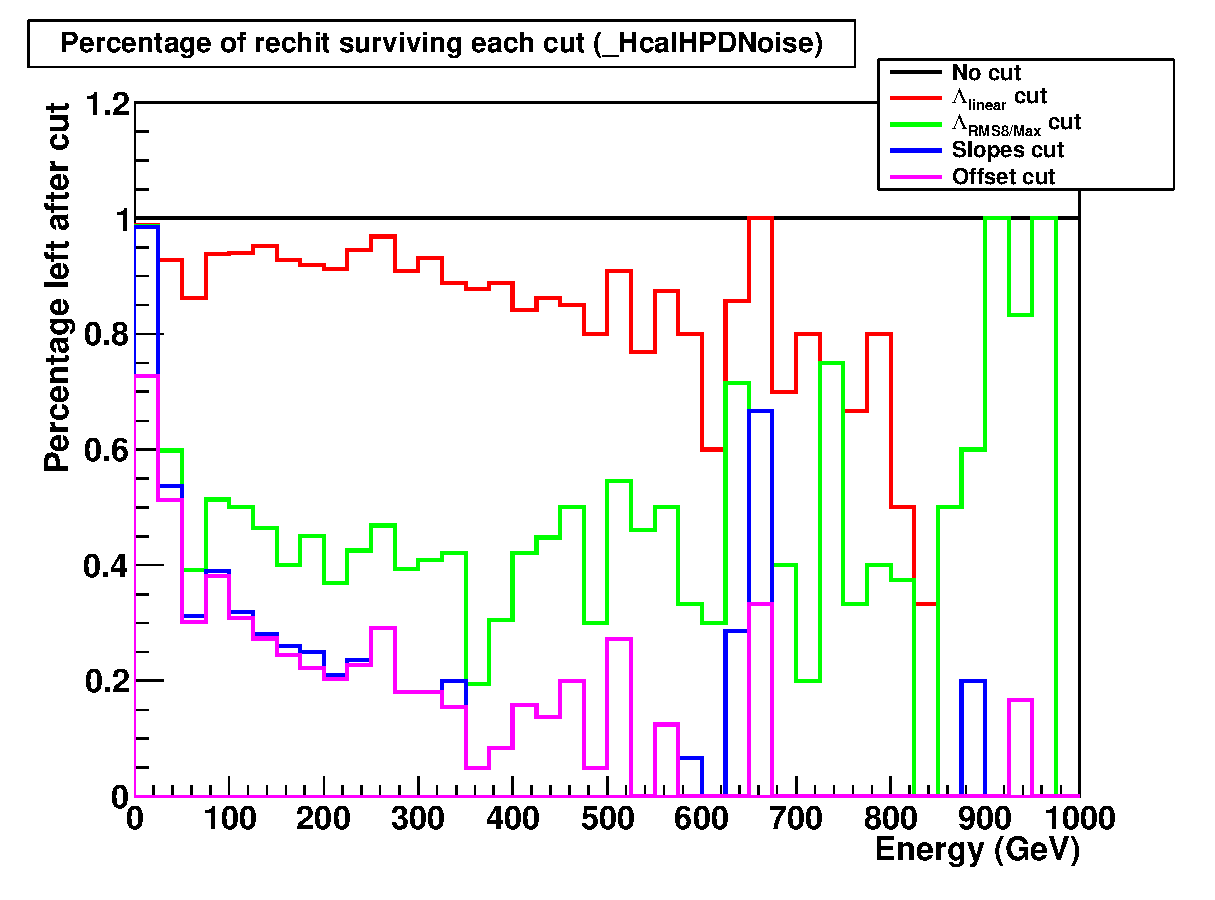
\includegraphics[width=120mm]{DailyLog/6363/6363_RecHitEnergyRatioPlot_HcalHPDNoise}
   \caption{Rate of pulse surviving each step of cleaning as a function of energy.  Note that the error bars are large for large energy rechits}
   \label{Figure_6363_RecHitEnergyDistributionCleaningRatio}
\end{figure}


